\chapter{Estado del Arte}

\subsection{Aplicaciones de rastreo para familia y amigos}

Actualmente las redes sociales forman parte de nuestra vida cotidiana, desde la posibilidad de enviar un mensaje privado, hasta la posibilidad de capturar en tiempo real nuestras historias y compartirlas con nuestra comunidad de amigos, entre muchas otras características. De esta manera las redes sociales ha logrado penetrar en lo más profundo del tejido social.

Así mismo, buscamos obtener la mayor experiencia de uso, apoyándonos de todas las posibles herramientas multimedia que existen. Tales como: texto, imágenes, voz, video, storytelling etc. y por supuesto recientemente el poder compartir nuestra ubicación en vivo con familiares y amigos.

De esta manera resolvemos la problemática que tenían los usuarios para reunirse en el mundo real. Ya sea que se esté compartiendo un viaje, que le informemos a nuestros seres queridos que hemos llegado a salvo, o reunirnos con nuestros amigos. Estas son experiencias muy comunes para todos nos otros. \cite{zafirKhan}

Es por  esto que las principales aplicaciones móviles han optado por  integrar esta caracteristica. 

Cabe mencionar que estamos aprovechamos el sistema de localización más exacto y preciso que existe y lo llevamos a nuestras interacciones humanas, para volverlas aún más emotivas y gratificantes.

\subsubsection{WhatsApp Live Location}

Según el articulo ``Digital 2019" publicado por Hootsuite (plataforma que permite gestionar redes sociales a nivel mundial) podemos observar el top de las redes sociales con más usuarios (actualizado a  en Enero del 2019). Figurando WhatsApp en el tercer puesto sólo después de Youtube y Facebook respectivamente, con 1500 millones de usuarios activos aproximadamente.\cite{kemp}

Al ser la red social líder en el servicio de mensajería instantánea surge la necesidad de agregar la característica de localización en vivo (tiempo real) con el objetivo de facilitar los encuentros personales en el mundo real con nuestros principales círculos sociales, familia/amigos.

La ubicación se comparte en cualquier conversación. Puede ser un chat uno a uno o un chat grupal.

Al abrir una conversación en la aplicación basta con presionar el ícono Adjuntar(Android)/Más(iPhone) donde tendremos incluida la opción: compartir ubicación. Tenemos dos opciones compartir la ubicación en tiempo real o simplemente la ubicación actual. Si elegimos la primera nos solicita agregar la duración de tiempo que permitiremos compartir nuestra ubicación (15 minutos, 1 hora(predeterminada), 8 horas). Si elegimos la segunda se enviara nuestra ubicación actual y sólo podrá verse de manera estática, es decir, sin actualización. En ambos casos nos da la opción de agregar un comentario, opcionalmente. Cabe aclarar que para la opción en vivo en cualquier momento se puede dejar de compartir la ubicación.

Los recursos compartidos de ubicación en vivo se mostrarán en los chats de WhatsApp como miniaturas que muestran la ubicación del usuario. Al tocar ‘Ver ubicación en vivo’ te llevará a una vista de mapa donde puedes ver la ubicación actual de todos los usuarios que actualmente comparten su ubicación en ese chat. Si lo desea, puede cambiar a una vista de Satélite / Terreno del mapa e incluso ver datos de tráfico en vivo como una superposición, lo que parece bastante conveniente si está esperando a alguien.

Debajo del mapa, se pueden ver los nombres de los mismos usuarios en una vista de lista, con una marca de tiempo, que indica la el lapso transcurrido desde la actualización más reciente de su ubicación. Podemos tocar un nombre en la lista o tocar una imagen de perfil en el mapa para ampliar la ubicación de un usuario en particular, donde podemos ver el posible margen de error (por ejemplo, "Precisión a 50 metros") para su ubicación. Así mismo podemos tocar el botón pequeño de información (se muestra con una 'i') que se encuentra al lado del usuario, para poder abrir una ventana emergente que nos permite comunicarnos con nuestro compañero, mediante WhatsApp de diferentes maneras.

En un grupo de WhatsApp, puede mostrar la información del grupo y ver a todos los usuarios que comparten su ubicación con el grupo en ese momento. Esto será particularmente útil en grupos más ocupados, ya que no tendremos que desplazarnos hacia arriba e intentar encontrar el mensaje donde el usuario compartió originalmente su ubicación.

Respecto al impacto en la duración de la batería, el actual product manager de WhatsApp Zafir Khan comenta: 

"Nuestro equipo de ingeniería pasó una cantidad significativa de tiempo optimizando la batería y el rendimiento de esta función". "Tenemos técnicas especiales para ayudar a conservar su batería cuando se comparte ubicación en vivo. Por lo tanto, tiene en cuenta una serie de factores diferentes, como el tiempo que ha estado compartiendo su ubicación en vivo, si alguien en el otro extremo con el que está compartiendo realmente está mirando el mapa, su nivel de batería actual".

"Tomamos en cuenta estos factores y muchos otros para determinar la frecuencia con la que se obtiene una actualización de ubicación desde su teléfono porque al ser inteligentes al respecto, podemos ayudar a conservar un poco de batería", agregó. "Acabamos de lanzar esta función, así que esto será algo que también optimizaremos continuamente con el tiempo a medida que obtengamos más uso de la función".\cite{zafirKhan}

Con todo esto podemos observar que la funcionalidad de compartir la localización en vivo con nuestros contactos de WhatsApp es realmente robusta, simple y práctica. Análisemos las ventajas y desventajas de la misma:

Ventajas:

1. Es una función robusta y optimizada.
2. Da soporte a la gran mayoría de smartphones que existen hoy día en el mercado.

Desventajas:

1. Excluye la funcionalidad de compartir la ubicación permanentemente, dejando de lado funcionalidades como almacenar un histórico de nuestra ubicación.
2. Al ser una aplicación de mensajería no está 100\% enfocada en el servicio de localización.

\subsubsection{Find My Friends - Apple}

Es una aplicación gratuita propiedad de Apple Inc. Está enfocada en la localización de familiares o amigos.

\begin{figure}[bp!]
	\centering
	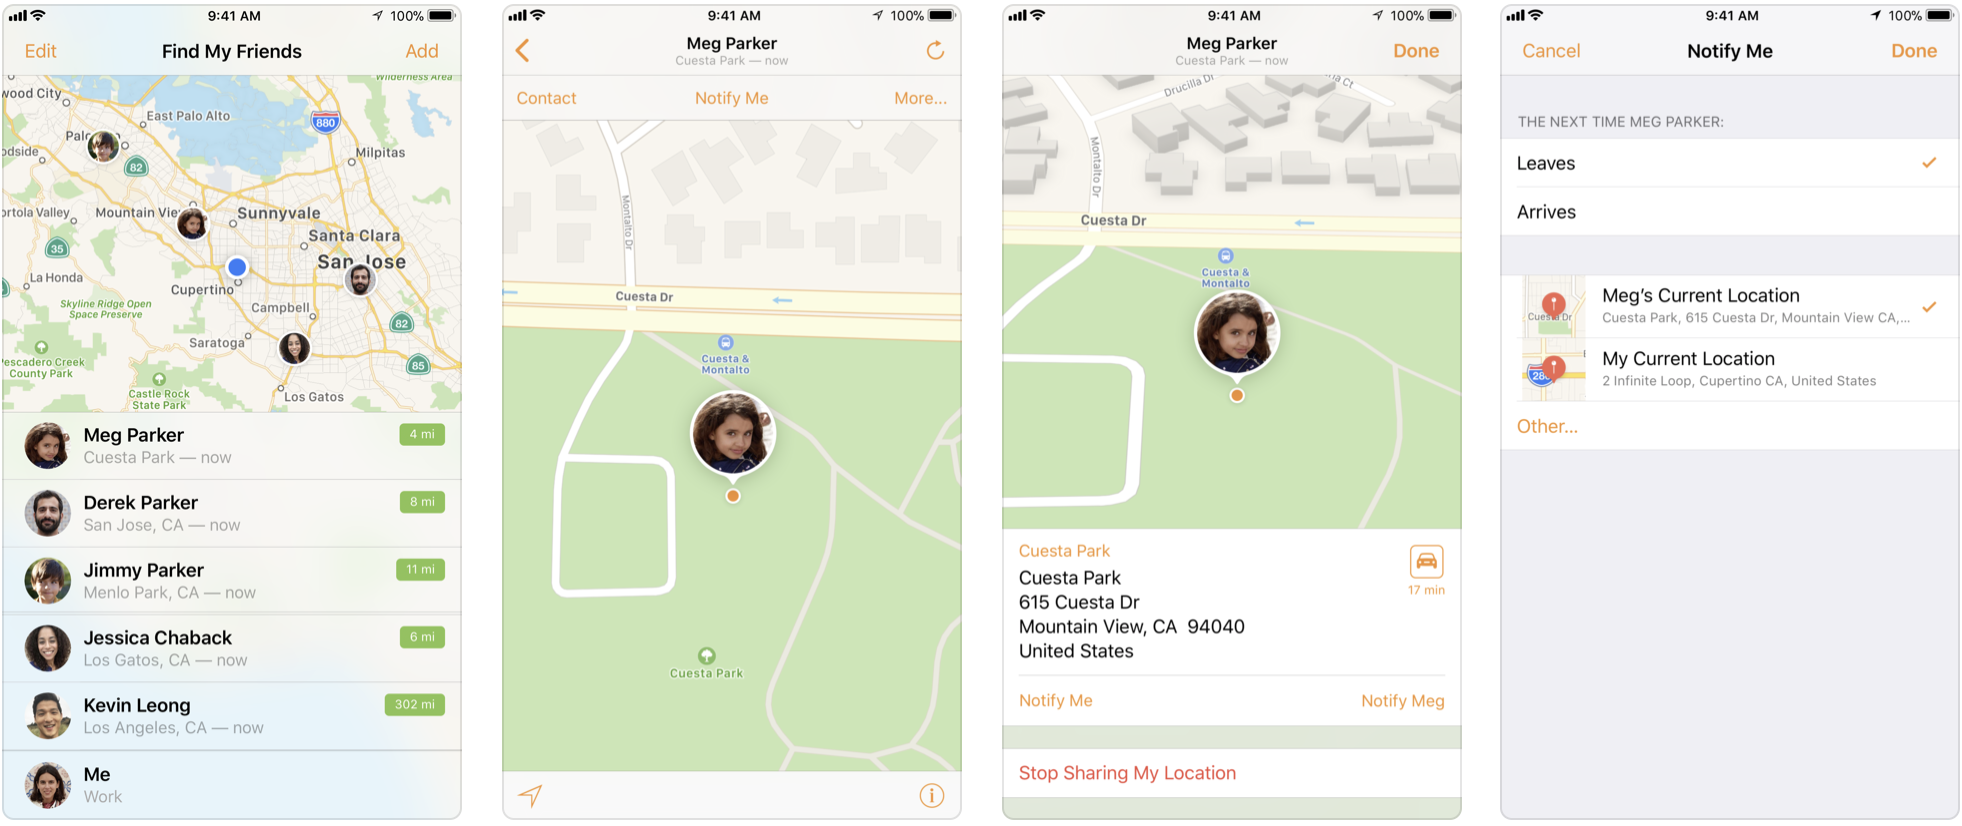
\includegraphics[width=5in]{imgs/apple_findmyfriends}
	  \caption{Find My Friends}
\end{figure}

``Find My Friends" version 7.0 requiere iOS 11 o posterior así como una cuenta de iCloud. Es compatible tanto para iPhone, iPad o iPod touch.

El primer paso es agregar contactos a nuestra aplicación enviando una solicitud a su dirección de correo asociada al iCloud del dispositivo, también es posible agregarlos a través de su número de teléfono igualmente asociado a su cuenta de iCloud o usando AirDrop (localizador de terminales Apple en un perímetro cercano, a través de bluethoot y la red wifi).

Posterior a eso tendremos que esperar a que acepte nuestra solicitud.

Una vez aceptada la solicitud ya forma parte de nuestros contactos. Ahora podremos compartir nuestra ubicación actual, así mismo nuestros contactos pueden empezar a seguir nuestra ubicación inmediatamente, también ellos pueden compartir sus ubicaciones. Si en algún momento se desea dejar de compartir la ubicación, basta con mover un interruptor para dejar de compartirla.

Una característica interesante y que agrega gran valor, son las notificaciones de geocercas (perímetros des algún punto/ubicación en especifico). Por ejemplo tiene la capacidad de notificar cuando un amigo llega al aeropuerto, cuando un niño sale de la escuela o un miembro de la familia llega a casa de manera segura. \cite{findmyfriends}

A continuación se muestran algunas ventajas y desventajas de la aplicación:

\paragraph{Ventajas}

\begin{itemize}
    \item ``Find My Friends" no almacena de manera permanente la información de nuestra ubicación.
    \item En la mayoría de los casos viene pre instalada.
    \item No necesita un registro ya que toma las credenciales de nuestra cuenta de iCloud asociada a nuestros dispositivo.
    \item Además de nuestra terminal física, se puede monitorear a nuestros contactos desde un navegador web, desde iCloud.com
    \item Se puede usar el Apple Watch (con WatchOS 3 o superior) para compartir la ubicación.
    \item Notificación de geocercas, entradas y salidas de nuestros amigos en un punto dado.
\end{itemize}

\paragraph{Desventajas}

\begin{itemize}
\item Tus amigos o familia deben tener un dispositivo Apple (iPhone, iPad, iPod).
\item En el día a día es común olvidar desactivar compartir ``ubicación", esto permite que tus contactos puedan ver tu ubicación actual permanentemente.
\item Si tus amigos dejan de compartir su ubicación, necesitas solicitarles compartan su ubicación y esperar a que lo hagan. Aun que se puede hacer desde la aplicación por lo general terminas solicitándolo desde otros medios.
\item Sólo un dispositivo envía la ubicación, es decir si tengo 2 iPhones y 1 Apple Watch sólo 1 de ellos puede compartir la ubicación con mis amigos. Sin opción de configurarlo.
\end{itemize}

En resumen al integrar todo el ecosistema de Apple se logra una gran calidad el funcionamiento de la aplicación, sin embargo también se vuelve muy dependiente de éste volviéndolo también su principal desventaja.